\chapter{Case Studies}
\section{Analyzing the power market structures and business opportunities in select cases}

PJM: symmetric (self-schedule, pool-auction), obligation (load contributing factor), market-based, imbalance(enforcement, 10\% waved for VRE),

Germany: asymmetric (balancing energy market vs frequency control market), 

AEMO: asymmetric (AEMO pays for provider, charge regulation from either all generators or all consumers, and charge contingency from causer)

\label{sec:qualitative-analysis}
The super-set of I is the set of selected energy market segments in different geographies:

\begin{equation*}
I \subseteq  \begin{cases}
\{Day~Ahead, Real~Time\} & PJM \\
\{Day~Ahead, Intraday, Balancing\} & Germany \\
\{Real~Time\} & NSW
\end{cases}
\end{equation*}

The superset of I is the set of selected reserve market segments in different geographies:

\begin{equation*}
J \subseteq  \begin{cases}
\{RegA, RegD, SR, NSR, DASR\} & PJM \\
\{PCR, SCR+, SCR-, TCR+, TCR-\} & Germany \\
\{Lower, Raise\} \times \{REG, 6SEC, 60SEC, 5MIN\} & NSW
\end{cases}
\end{equation*}

\subsection{PJM}
\subsubsection{Organization of PJM power markets}
Marketplaces
Timeline

\subsubsection{Players}
A Load Serving Entity (LSE), as is defined officially by PJM, is "any entity that has been granted authority or has an obligation pursuant to state or local law, regulation, or franchise to sell electric energy to end-users that are located within the PJM RTO. An LSE may be a Market Buyer or a Market Seller"\cite{PJM2017b}. Therefore, LSEs refer to all market participates in PJM who have rights and obiligation to act in all the power marketplaces of PJM, including the energy, capacity and ancillary services markets. 

Curtailment Service Providers (CSPs) are members in PJM markets specializing in demand response. A CSP is an intermitted agency that provides the end-user DR to the wholesale market. \cite{PJM2017b} \cite{Wang2015} The role of the CSP is actually a legacy product from the liberalization of retail markets in PJM. Once the retail competition began, PJM allowed LSEs to provide DR not only for their own customer but also for customers of other LSEs. The role of the CSP was created to facilitate the liberalization and competition. \cite{PJMInterconnection2017}

\subsubsection{Balancing mechanism}
submit offer - rebid - update information up to 65 mins - deviation charged with real-time

reviewed the participation, violating -> suspend activity, enter enforcement

LSE obiligate to purchase (or self-schedule) reserve, obiligation as a proportion to its contributing flow to the grid. \cite{PJM2017c} This incents liquidity in the market with competitions on both buyer's and seller's side. However, the obiligation does not reflect their actual needs.\cite{Wartsila2014}

CSP
intermitted agency
allowed to voluntarily respond to the LMP

\subsubsection{PJM DR}

PJM DR is the umbrella for all distributed energy resources, including DR, behind-the-meter generations, storage, etc. since PJM does not specify how the load is reduced. However, PJM DR program does not allow energy injection beyond the meter and receive wholesale compensation.\cite{PJMInterconnection2017}. This issue is currently under discussion in Special Market Implementation Committee meetings.

DR emergency fast changing over years \cite{Brown2015}
Since the DR in the wholesale market as a supply recouse will cause double payment issue where a customer may receive wholesale energy revenue and retail cost savings for the same MW of load reduction, PJM states that DR participation in the retail market on the demand side would be more ideal. And they are discussing to revisit the mechanism. Therefore, this value is not fully modeled in our study.

LSE
buyer or seller in Energy, and reserve market

\subsubsection{Identify business model}

\subsubsection{Accounting}





The real-time market price is applied for all deviations from day-ahead planned schedule, including Regulation, Primary and Supplementary Reserves.

\begin{equation*}
\pi_t^{e,j} = \pi_t^{e,i} ~~~~ i \in \{Real~Time\}, j \in \{RegD, RegA, SR, NSR, DASR\}
\end{equation*}

The capacity prices of reserves are computed using a complex algorithm, taking into account a list of specifications of the resrouce, e.g. the performance \& historical performance, benefits factor, milleage, etc. The detailed calculations can be found in appendix. As outputs, we will get deterministic values for $j \in \{RegA, SR, NSR, DASR\}$, and the upper and lower bounds, $\overline{\pi}_t^{r,j}$ and $\underline{\pi}_t^{r,j}$, for $i \in \{RegD\}$.

%Reg = RMCCP + RMPCP + LOC
%LOC = 0
%RMCCP = 
%RMPCP = Milleage
%Effective MW = BF * MW
%BF is determined with the average and upper, lower bounds

\subsection{Germany}
$\pi_t^{e,i}, i \in \{Balancing\}$, is the the price for balancing energy (reBAP), which exist only in Germany

$\pi_t^{r,j}$ and $\pi_t^{e,j}$ are based on principle of pay-as-bid. The weighted-average values are available in the datasets.

%Market participants in Germany are organised into balancing groups, known as Bilanzkreise (BK). BK can range from individual large generators to aggregations of smaller renewable generations, to a Stadwerke representing large portions of aggregated demand.

%Every balancing group operator is responsible for following a planned schedule with a 15-minute resolution. Deviations from the planned schedule are balanced physically by the TSOs and settled financially with the BK. There is a legal obligation on Bilanzkreise to balance their positions to the best of their ability.

Prices for balacning energy are unified across TSOs and determined according to the  balancing energy price settlement system (BK6-12-024) developed by Federal Network Agency (FNA) as of 01/12/2012.

\begin{equation}
\label{eq:reBAP}
reBAP = \frac{\sum net imbalance energy cost}{\sum net imbalance energy volume}
\end{equation}

\subsection{Australia-New South Walse}
The unit prices of reserve products, $\pi_t^{r,j}$ and $\pi_t^{e,j}$, are not available in datasets published by AEMO. Only weekly summary for total payment and recovery are provided. Due to the limits of available data, we are only able to perform calculations of total potential revenues, rather than thorough studies as in the other two geopraphies.

\section{Accounting rules and electricity market data preparation}
\label{sec:accounting-data-prepare}
\newpage

\section{Quantitative studies and results}

\subsection{Value of markets with current market conditions}
We first examined the value of markets for flexibility management under current market conditions, i.e. based on historical observations without involving the market simulation module (Section \ref{sec:market-simulation}). The impact of possible changes in market conditions such as renewable penetration will be discussed later in Section \ref{sec:impact-market-condition}.

The electricity market data in this section corresponds to the actual market data from January 1st 2016 to December 31st 2016 and were pre-processed according to different accounting rules in different geographies as is described in Section \ref{sec:accounting-data-prepare}.

For cost determinations, we would first use figures based on the present market pricing level, and then make scenarios with reduced costs to find the break-even point if it is not yet profitable. According to the International Renewable Energy Agency\cite{IRENA2017}, the cost for battery energy storage systems was analyzed as proportional to their energy capacity, $\overline{s}$, and the energy cost coefficient, $C^s$, for state-of-the-art lithium-ion batteries were reported to be ca. $\$350/kWh$ in 2016. The replacement cost were based on actual price from Tesla\cite{Tesla1}, one of the leaders in battery and electric vehicle markets. The operating life is set to be 6000 FCEs, which corresponds to an optimistic estimation by Sandia National Laboratories\cite{Akhil2015}. Designed life time is assumed to be 10 years. Discount rate is made as 10\% as is discussed in Section \ref{sec:cost}. The technology costs were made to be zero so that the derived profits will be the margins that can be possibly realized by technology vendors. All the parameters for cost calculation are summarized in Table \ref{table:cost-parameters}. 

\begin{table}[h!]
	\label{table:cost-parameters}
	\begin{center}
		\begin{tabular}{| l | l | R{2.7cm} |} %R{2.7cm} |}
			\hline
			\textbf{Items} & \textbf{Unit} & \textbf{Value} \\% & \textbf{Reduced Cost} \\
			\hline
			\hline
			Energy cost coefficient, $C^s$ & $\$/kWh$ & 350 \\%& 140 \\
			\hline
			Power cost coefficient, $C^r$ & $\$/kW$ & 0\\% & 0 \\
			\hline
			Technology cos,t $C^0$ &$\$$ & 0\\% &0\\
			\hline
			Replacement cost coefficient, $C^s$ &$ \$/kWh$ & 150\\% & 60 \\
			\hline
			Designed life time & \textit{year} & 10\\% \multicolumn{2}{c|}{10}\\
			\hline
			Operating life time & \textit{FCE} & 6000\\% \multicolumn{2}{c|}{6000}\\
			\hline
			Discount rate &$\%$ & 10\\% \multicolumn{2}{c|}{10}\\
			\hline
		\end{tabular}
	\end{center}
	\caption{Parameters for cost calculation}
\end{table}

It shall be pointed out that by using the parameters described above, the ESSs are virtually battery energy storage systems (BESSs). This fits the purpose of case studies. However, the conclusions on profitability are not portal for other types of ESS, but it does not mean the methodology loses its generality. The value of revenue would still be valid for other types of technology as long as they can have the same function as BESS. Furthermore, by using different data as inputs, our model can be utilized for analysis of profitability of other energy storage systems with different cost dynamics. 

In terms of EV2G studies, we first determined the battery parameters of EVs.

\begin{itemize}
	\item EV charging rate is 10kW, corresponding to the guidance provided by Tesla\cite{Tesla2} and a typical home charging infrastructure with 50A current limit. 
	\item The battery energy capacity per EV of 75kWh is taken from one of the most popular EV models\cite{Tesla3}.
\end{itemize}

Simulations are then performed to get EV driving profiles, which are based upon data from the California Department of Transportation's California Household Travel Survey for 2010-2012\cite{NREL_TSDC}. This survey carried out multiple objectives and included 79011 vehicles. For our work we focus on a proportion of the vehicles, 2910, which were fitted with GPS. These vehicles were monitored continuously for a 7-day window with the 1-second resolution. The GPS data is then processed into trip profiles, while include information of the location of each EV at each time step as well as the trips made by each EV. Furthermore, together with the parameters of the EV model we have selected above we simulated the SoC time series of the EV batteries. Finally, from the simulated results, we can statistically derive the value of probability distribution of EV plug-in $n^+$, plug-out $n^-$, and average state-of-charge (SoC) of batteries plug-in $s^+$, plug-out $s^-$, as introduced in Section \ref{sec:tech-simulation-module}. The results are shown as Figure \ref{fig:data-ev-number}-\ref{fig:data-soc}.

\begin{figure}[h!]
	\centering
		\centering
		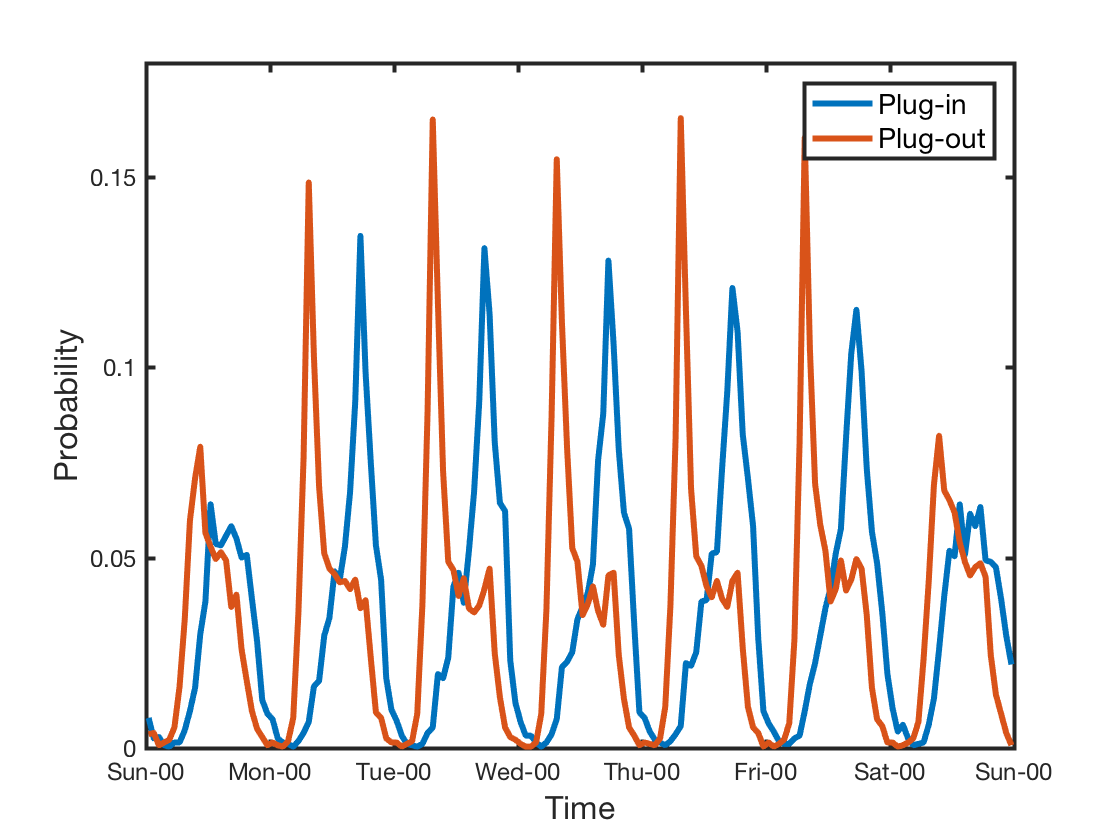
\includegraphics[width=0.8\linewidth]{Figures/Data_EV_number}
		\caption{Probability of EV plug-in/ plug-out}
		\label{fig:data-ev-number}
\end{figure}

\begin{figure}[h!]
	\centering
		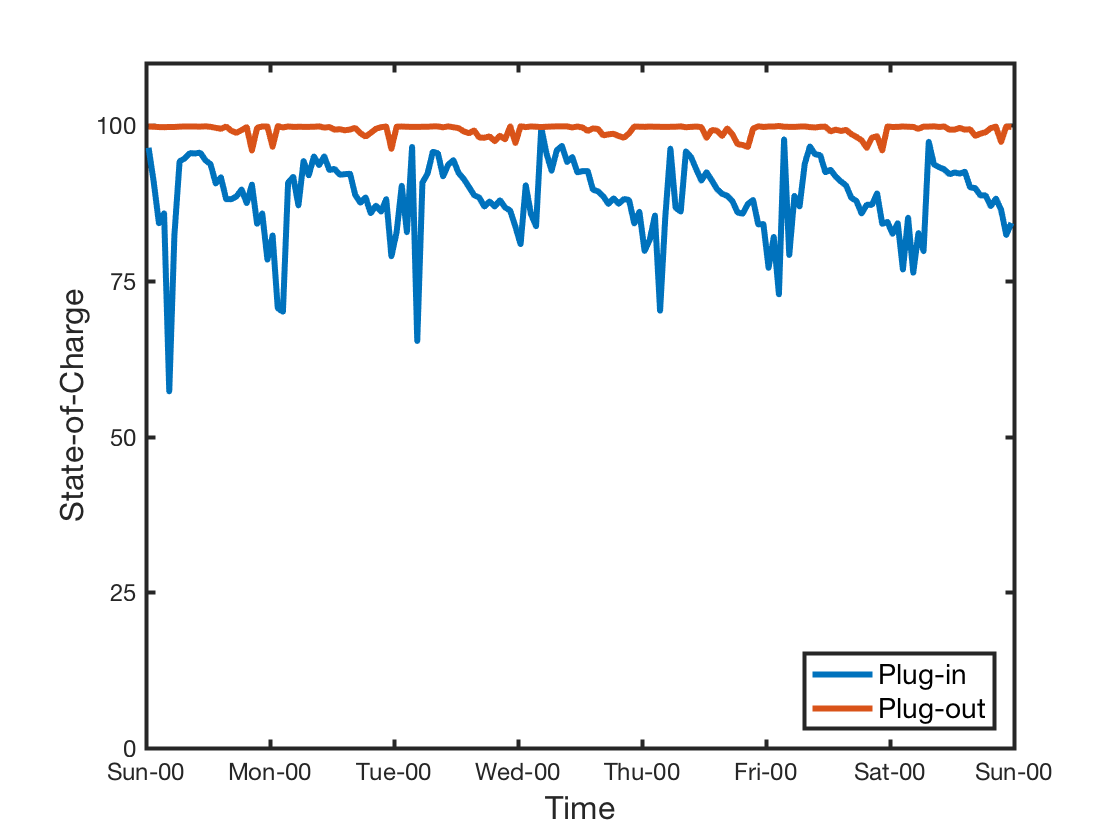
\includegraphics[width=0.8\linewidth]{Figures/Data_SoC}
		\caption{Average SoC of EV when plug-in/ plug-out}
		\label{fig:data-soc}
\end{figure}

The metrics to evaluate the system performance are slightly different between ESS and EV2G. For ESS, the criteria in the evaluation metrics include
\begin{itemize}
	\item \textbf{Revenue:} the total explicit revenue from electricity markets calculated as Equation \eqref{eq:module-revenue}
	\item \textbf{Operating Profit}: the total revenue net of operation-dependent costs (degradation cost)
	\item \textbf{Profit:} the total revenue net of both operation-dependent and fixed costs
\end{itemize}

For EV2G, the fixed cost that is mainly related to procuring the battery stocks shall not be considered for a technology vendor. Furthermore, the implicit charging cost to compensate the energy consumed by EV driving are listed separately. Depending on the specific business model in practice, a portion of the implicit charging cost may be recovered by the technology vendors from the end-users, although in this thesis we did not exclude it from calculating the profit. As a result, the criteria are altered as:
\begin{itemize}
	\item \textbf{Revenue:} the total explicit revenue from electricity markets calculated as Equation \eqref{eq:module-revenue}
	\item \textbf{Implicit Charging Cost}: the cost of energy compensation for EV driving demands, calculated as the total energy consumption multiplied by average price over the span of one operational cycle
	\item \textbf{Profit:}: revenue net of costs including the implicit charging cost and battery degradation. The investments on technology are made to be zero as is discussed at the beginning of this section
\end{itemize}

As a result, the profit of a EV2G system is closed to the concept of operating profits for a ESS, which excludes the investment of procuring batteries. This implies two disparate business models. Cautions shall be raised while comparisons between these two technologies are made.

In order to determine the market size and profitability of ESS, we evaluated the system performance with different total sizes. Thereafter, we would select and analyze 4 key states corresponding to 4 scenarios as following:

\begin{itemize}
	\item ``\textbf{max. Revenue}": the state where the maximum potential revenue is extracted from the markets. The ``max. Revenue" state is determined as when the marginal increment of revenue is less than 5\% with additional system capacity, i.e. 
	\begin{equation*}
	\frac{\Delta\text{Revenue}}{\Delta\text{System Size}} < 0.05
	\end{equation*}
	Since in our studies, we found the operating profits are always in line with revenue, so this state is equivalent to``\textbf{max. Operating Profit}".
	
	This scenario can present a reference of the maximum market potential to technology vendors as they might be able to develop technologies with lower costs than what we calculated in the case studies. 
	\item ``\textbf{max. System Size with pos. Profit}": the state indicating maximum possible system size where the profit is barely above zero. Since in our studies the profits either drop monotonically or decrease after an initial rise, this state is obtained when the profit falls to be 0.
	
	This scenario would inform technology vendors about when the market would be saturated. Without revolutionary innovations on technologies or drastic changes on market conditions, expanding the flexibility fleet beyond this scenario is likely to create losses rather profits. 
	
	\item ``\textbf{max. Profit}": the state where the profit is maximized.
	
	If the total system size goes beyond this scenario, it indicates that the competition will intensify and the profit will drop with additional market entrants.
   
	\item ``\textbf{max. marginal Revenue}": the state where the marginal increment is maximized. 
	
	This scenario is presented to allow the readers to have a more intuitive understanding about the maximum potential return per unit system.
	
\end{itemize}

The 4 scenarios can be illustrated by Figure \ref{fig:scenario-illustration} using the results from a case of making arbitrage in day-ahead, real time energy markets and simultaneous delivering regulation services in PJM electricity markets.
\begin{figure}[h!]
	\centering
	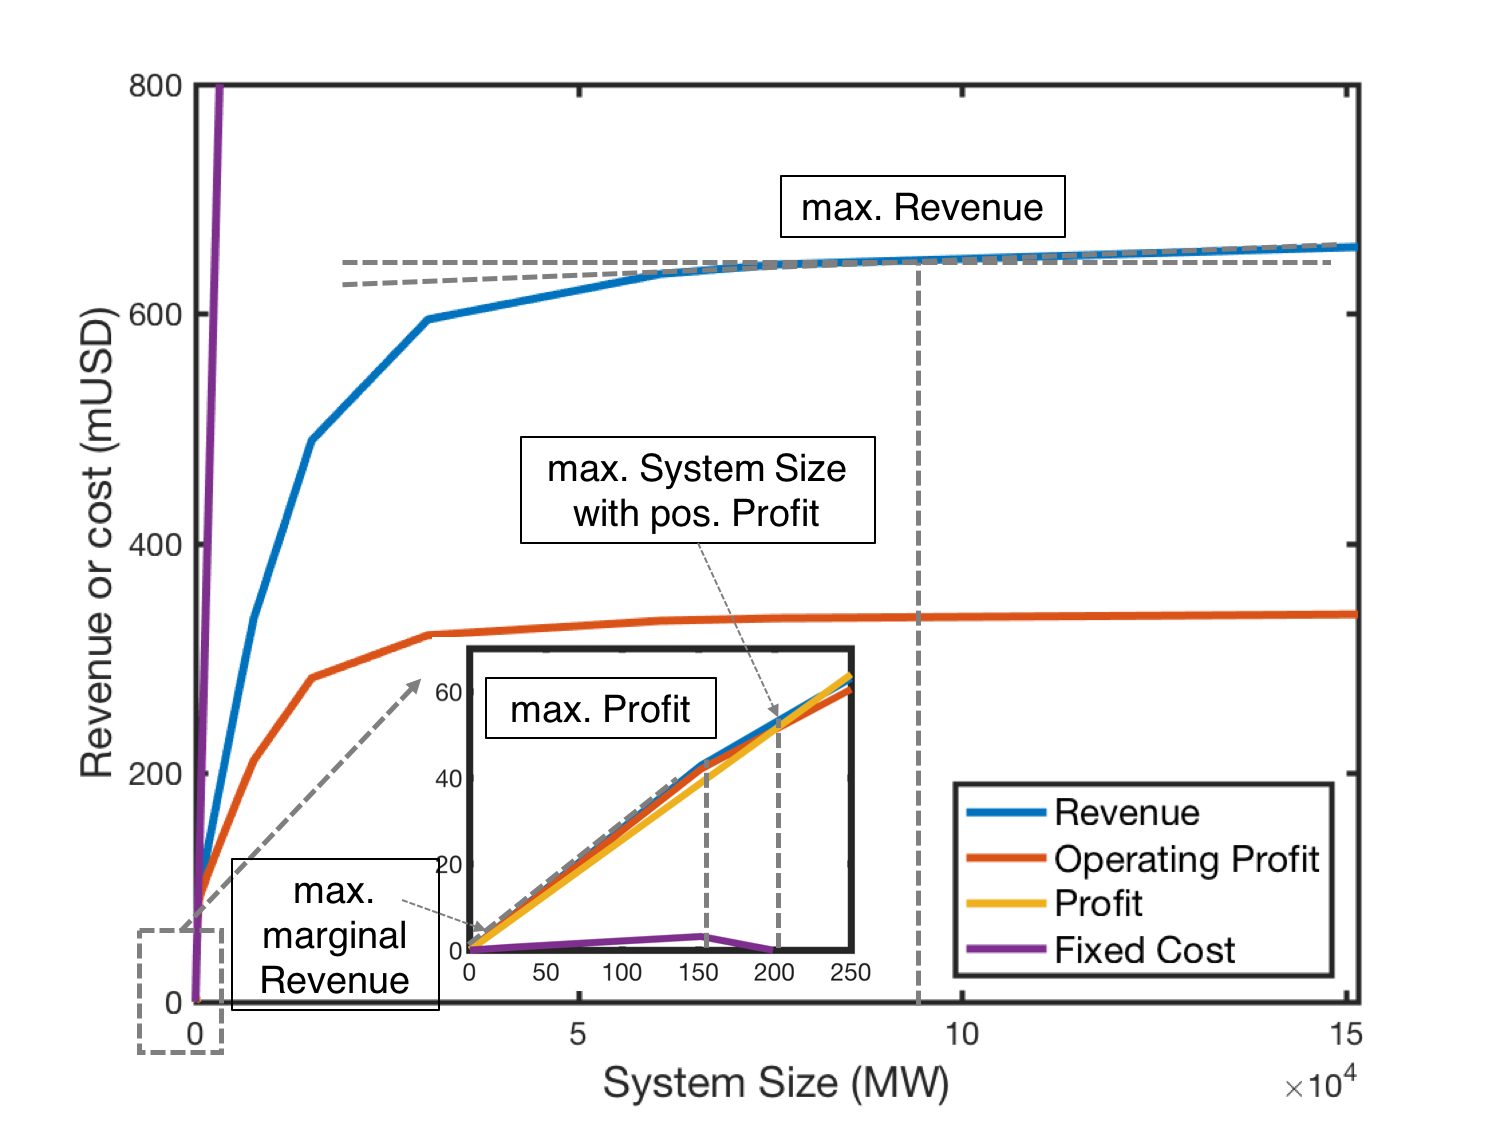
\includegraphics[width=0.95\linewidth]{Figures/Scenario_illustration}
	\caption{Graphic illustration of 4 scenarios}
	\label{fig:scenario-illustration}
\end{figure}

In terms of EV2G, the size of the system (number of EVs) are not strongly related to the profitability of EV2G, if at all. Therefore, it makes no sense to analyze the optimal system size in relation to the profitability. Instead, we would show the market values under certain scenarios where the number of EVs is determined externally. 

Finally, the overall scale of the market in a geography is represented according to the metering points (MPs). We would refer to the value per MP to make cross-regional comparison. The statistics are provided by commercial market data provider, Northeast Group\cite{NortheastGroup2016}\cite{NortheastGroup2017}\cite{NortheastGroup2017a}, and listed in Table \ref{tab:MP}.

\begin{table}
	\label{tab:MP}
	\centering
	\begin{tabular}{| l | R{2.7cm} |}
		\hline
		\textbf{Geography} & \textbf{MP} \\
		\hline
		\hline
		Germany & \num{51869730}\\
		PJM & \num{30331401}\\
		NSW & \num{3364428}\\
		\hline
	\end{tabular}
\caption{The number of metering points in each geography}
\end{table}

The currency exchange rates are determined as the real market data as of January 1st 2018, when 1 EUR is equal to 1.20 USD and 1 AUD is equal to 0.78 USD\cite{Bloomberg}.

\subsubsection{Market size and profitability of ESS in Germany}
Figure \ref{fig:germany-ess} summarizes the market size and profitability of all cases for ESSs in Germany electricity markets. 

\begin{figure}[h!]
	\centering
	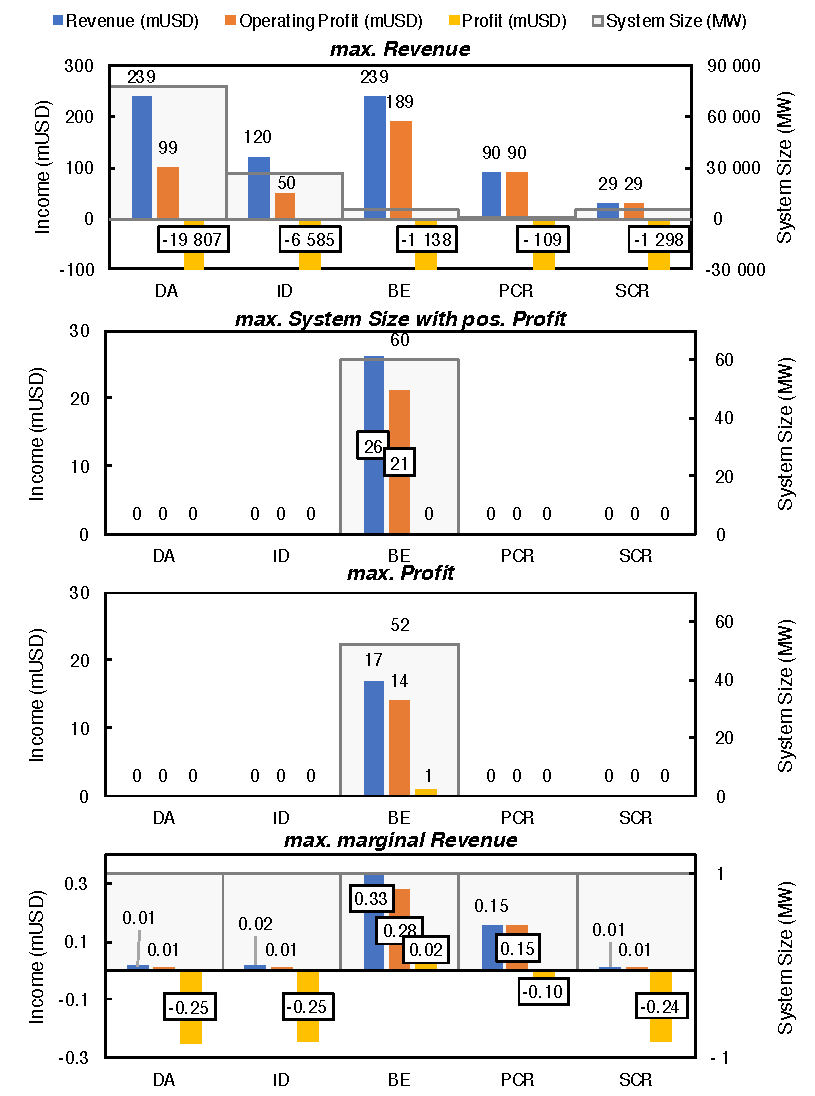
\includegraphics[width=0.9\linewidth]{Figures/Germany_ESS}
	\caption{Market Size and Profitability of ESS in Germany Electricity Markets}
	\label{fig:germany-ess}
\end{figure}

It was found that the only profitable case is delivering balancing energy. As is analyzed in Section \ref{sec:qualitative-analysis}, this case corresponds to the situation of self-balancing where the players turn to the flexibility resource in avoidance of charges by TSOs for their imbalances. 

It can be seen from Figure \ref{fig:germany-ess}, if being operated optimally BESSs with a overall size of up to 60MW can generate profits by serving balancing energy. Nevertheless, it is challenging to be realized in practice. Market players do not have the right information to optimize their operational plans, since the balancing energy price, reBAP, is calculated \textit{ex-post} and highly volatile, hardly predictable, as is discussed in Section \ref{sec:accounting-data-prepare}. On the contrary, if a system is designed to be just ``large enough" and tackle almost all imbalance events, it corresponds to a situation as the ``max. Revenue" scenario where we see negative profits.

On the other hand, we noticed that selling frequency control service to TSOs is less economically viable than using BESSs for self-balancing. Under same system size, the revenue from self-balance is significantly higher than from selling frequency control products, while ideally the situation shall be reversed. The balancing energy charges are designed to recover the costs of activating frequency control services (calling for energy delivery) while the costs paid for securing capacity commitment are socialized, as have been fully discussed in Section \ref{sec:accounting-data-prepare}. Theoretically, players shall get higher turnover in the frequency control markets than avoided balancing energy charges. Our results imply that the current design of frequency control markets is not economically efficient to integrate the emerging BESS resources, which verifies our analysis in Section \ref{sec:qualitative-analysis}. We have argued that hurdles exist against emerging BESS to participate in frequency control markets with the non-energy-neutral signals and block-wise offering, especially for SCRs which demand significantly higher energy delivery than PCRs.

Facing either lack of information transparency in balancing energy charges or unfavorable market rules in frequency control markets, BESS players have no feasible options in the current market setup to make profits.

However, we may argue this situation shall not be long-lasting. We have already see that certain amount of BESS will be a cheaper option to defer the expense on imbalance settlements compared to what are currently incurred. The market operators shall develop well-designed framework to encourage the participation of these resources that are beneficial to lower the overall system costs. In reality, there are indeed debates proposing possible solutions on this issue, e.g. letting TSOs who have the most abundance of information own and dispatch the storage resources\cite{He2012}, re-engineering the pricing mechanism of balancing energy\cite{Wartsila2014} and implementing favorable frequency control products for storage\cite{Megel2017}, etc.

As an implication for technology vendors, these possible movements on market designs shall be taken care of as it could suddenly turn over the feasibly profitability of using BESSs for balancing services.

Regarding arbitrages value in energy market, although the potential revenues are 239 mUSD/a in day-ahead and 120 mUSD/a in intra-day market, the losses would be incredibly high in order to materialize the revenue using BESSs. Even in the scenario of maximum unit return, the losses are about 10-20 times of the revenue. It is clear that the heavy investments on batteries cannot be recovered from making arbitrage in energy market. However, since the operating profits are always positive, if technology vendors can enable similar functions as BESS using technologies with smaller capital costs such as certain types of DR, it is still possible to make profits out of the market worth over 300 mUSD per annum.

As has been discussed qualitatively, in order to increase the profitability and find a way to neutralize the frequency control signals, we may stack operations in day-ahead, intra-day and secondary control reserve for multitasking. Figure \ref{fig:germany-ess-multitasking} shows the effects of multitasking.

\begin{figure}[h!]
	\centering
	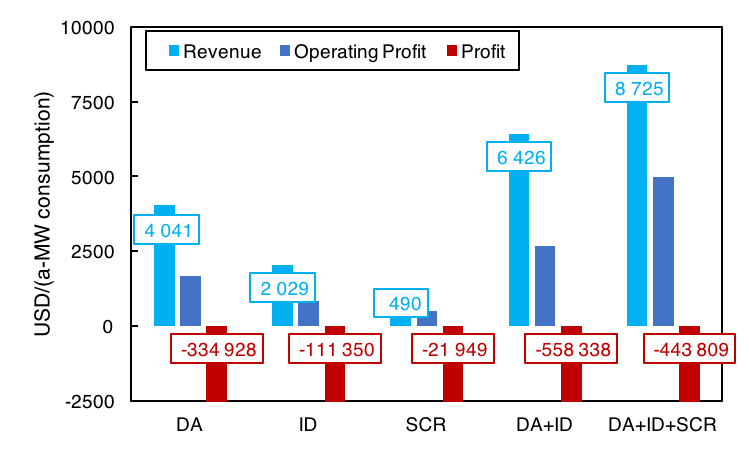
\includegraphics[width=0.95\linewidth]{Figures/Germany_ESS_multitasking}
	\caption{Market Size and Profitability of ESS with multitasking in Germany Electricity Markets}
	\label{fig:germany-ess-multitasking}
\end{figure}

While there are no significant synergies between day-ahead and intra-day markets, stacking secondary control reserve with these energy marketplaces will significantly improve the unit return as well as the maximum revenue potential. This corresponds to our previous analysis that the issue of non-energy-neutral signals can be tackled by introducing third-party energy for offset. Nonetheless, these  two cases with multitasking are still not profitable.

To sum up, technology vendors shall consider other technologies than BESSs or expect drastic cost reduction of BESSs to unlock the arbitrage value worth over 300 mUSD/a in Germany. Profits from balancing market are more technically tangible, yet adjustments on market frameworks are required.

\subsubsection{Market size and profitability of ESS in PJM}
The results of case studies in PJM power markets are illustrated in Figure \ref{fig:pjm-ess}.
\begin{figure}[h!]
	\centering
	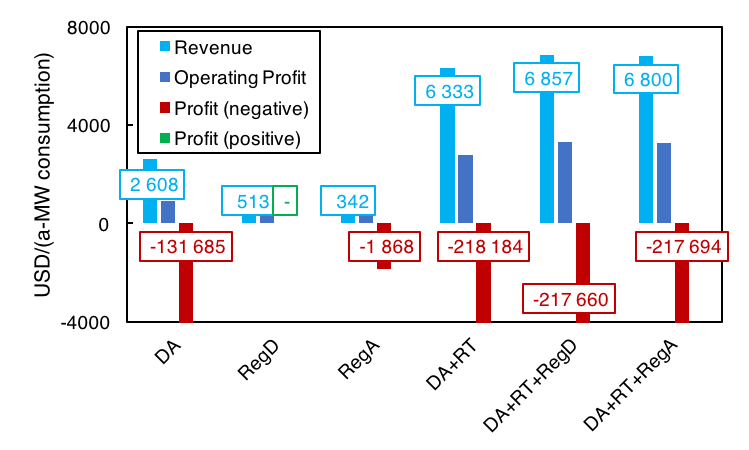
\includegraphics[width=0.9\linewidth]{Figures/PJM_ESS}
	\caption{Market Size and Profitability of ESS in PJM Electricity Markets}
	\label{fig:pjm-ess}
\end{figure}
As we can clearly see, the RegD marketplace that is specially designed for emerging flexible technologies is indeed profitable. By implementing energy-neutral signals as well as introducing concept of mileage ratio and beneficial factor to shift the RegD price against RegA, the market with a total size of 45 mUSD can be materialized by 154MW BESSs without writing a loss, although the margin is very niche, barely above zero. 

Stacking it with the energy market does not significantly improve the profitability. The energy-neutral signals allows a BESS to sustain the provision of RegD service over a period without involving transactions in energy markets. The advantage of multitasking in this case is only to allow the decision makers to have more choices so that they can better schedule their plan by responding to the price trend. PJM allows participates to alter their RegD offers in hourly block which grants additional operational flexibility compared to the arrangement in Germany's frequency control markets. However, as we can see from Figure \ref{fig:pjm-multitasking}, RegD is preferred due to its higher profitability and resources are rarely allocated to deliver day-ahead or real-time energy in the optimized plan.

\begin{figure}[h!]
	\centering
	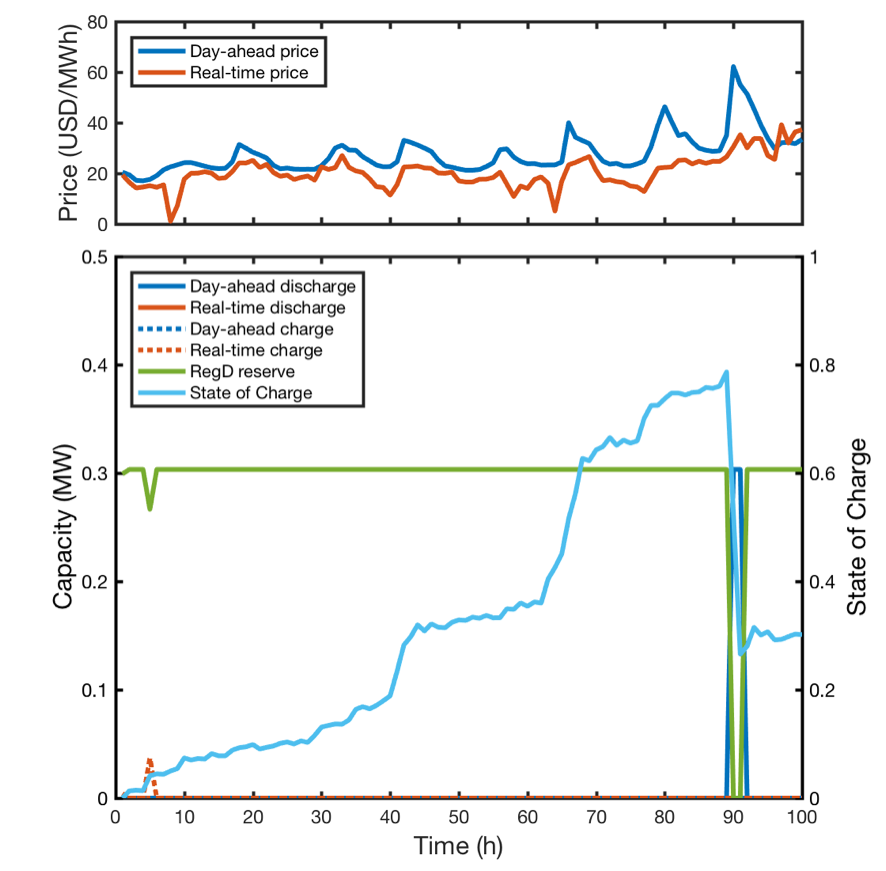
\includegraphics[width=0.9\linewidth]{Figures/PJM_multitasking_example}
	\caption{A example of operational plan with a 0.3MW battery energy storage system}
	\label{fig:pjm-multitasking}
\end{figure}

Apart from RegD market, there are no other profiting opportunities existing in PJM. Even the conventional regulation service RegA will create losses to BESS players.

Arbitrage in the energy market with flexibility through the so-called economic DR program, as is discussed in Section \ref{sec:qualitative-analysis}, is deemed not an ideal choice, especially in recent years when the electricity prices had fallen drastically with the shell gas revolution. As is discussed in Section \ref{sec:qualitative-analysis}, participating in the emergency DR program is a better option. However, the involvement of capacity market is not within our scope of quantifying the value, but the profiting mechanism is straightforward as is fully explained in the qualitative analysis.

\subsubsection{Market Size and Profitability of ESS in NSW}
In New South Wales power markets, we only studied the real-time energy market due to the limitation of data availability. Only information about total payment are available for the frequency control products. The total payment in these unaddressed markets is worth 23.4 mUSD in 2016, which are significantly smaller compared to the total payment in the real-time energy market that is 8.7 bUSD, and even much lower than merely the arbitrage value of over 1.8 bUSD/a as shown by Figure \ref{fig:nsw-ess}. This reflects the philosophy of market design that the real-time energy market is fully exploited to response to the system imbalances which are otherwise tackled by frequency control markets\cite{AEMO2010}\cite{McConnell2015}. This also explains the fact that the arbitrage value is 3-5 times the maximum arbitrage revenue in the other markets in absolute value and 30-75 times higher while normalized to their metering points.

Nonetheless, even though the total arbitrage potential is much higher and the operating profit per unit is also about 6 times the values in the other geographies, it is still not a profitable business to deploy BESS.

\begin{figure}[h!]
	\centering
	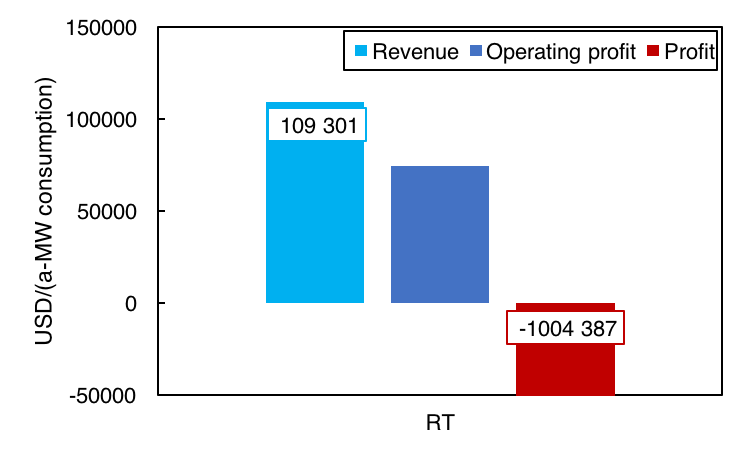
\includegraphics[width=0.9\linewidth]{Figures/NSW_ESS}
	\caption{Market Size and Profitability of ESS in NSW Electricity Markets}
	\label{fig:nsw-ess}
\end{figure}

\subsubsection{Impact of cost reduction}
According to the results above, using BESSs for balancing is already technically feasible while limitations lie in the aspect of market design. The value of arbitrage is far away from profitable due to expensive battery prices. Moreover, there are no evidences 
Overturn of profitability will rely exclusively cost, market condition

\textit{(This subsection will come later. As a short summary, only PCR in Germany and RegA in PJM switched their profitability to be profitable. The other cases of arbitrage that were shown to be unprofitable still lead to losses even with the cost reduced by 60\%.)}


\subsubsection{Market Size and Profitability of EV2G  in Germany}
Implementing EV as a grid resource is not as straightforward as using a generic ESS that is discussed above. The main issue is that the energy demand for EV driving itself poses challenges to grid. It is not possible to deliver any services without incorporate a large-volume energy market. Therefore, the day-ahead energy market is always included for all the cases for EV2G. Moreover, in our case studies, it is found even with the day-ahead market, charging the EVs is not feasible while their number reached a certain level. In the optimization framework, the technology constraints would violate market constraints with large number of EV fleet, especially the one that we set to restrict the activation of peak generation during non-peak hours. This corresponds to the situation that spare generation resources in the power system are not sufficient  to fulfill the energy needs of EVs. The electricity price may raise significantly in those scenarios compared to nowadays. As is shown by Figure \ref{fig:EV_nan_percentageg}, when the number of EV is higher than 1 million, it start to stress the electricity supply with present generation fleet. 
\begin{figure}[h!]
	\centering
	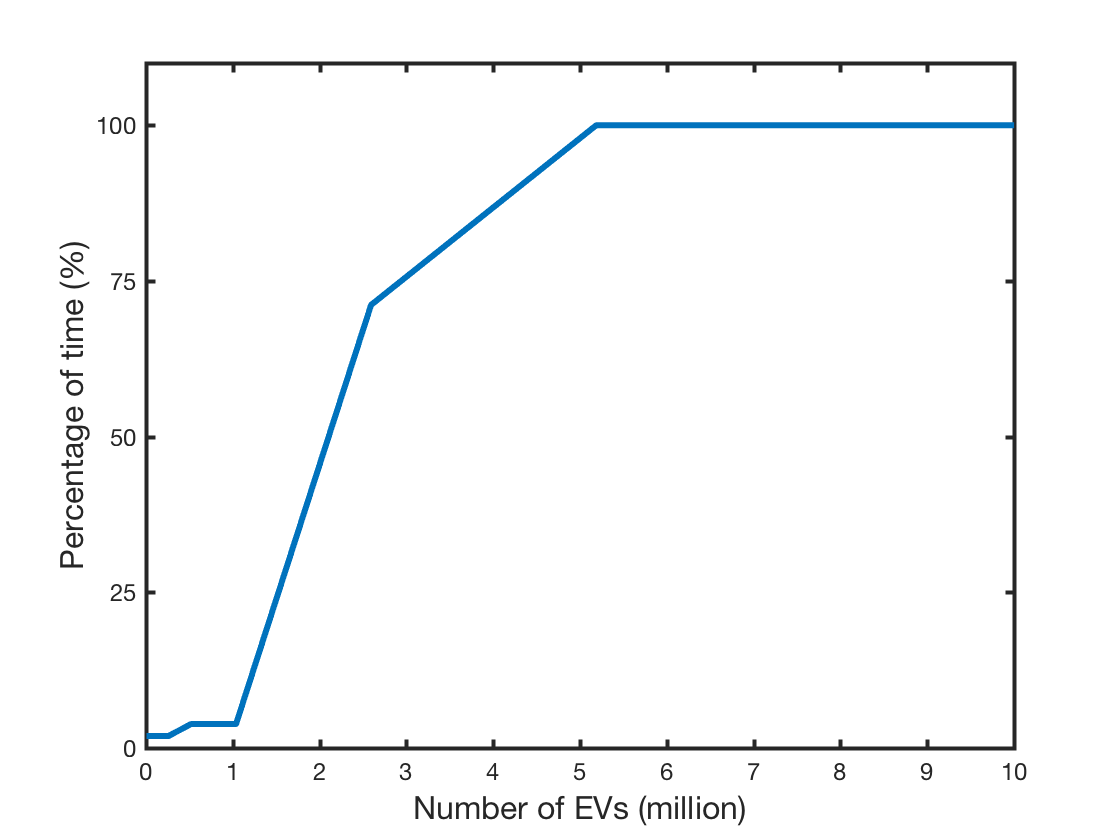
\includegraphics[width=0.95\linewidth]{Figures/EV_nan_percentage}
	\caption{Percentage of time when EV charging demand cannot be fulfilled in Germany}
	\label{fig:EV_nan_percentageg}
\end{figure}

This finding implies when there will be 1 million more EVs in Germany compared to the level in 2016, it will create great incentives for infrastructure extension of electricity grid, which reveals a promising business opportunity. Nevertheless, studies under that condition is beyond the focus of our work.

In this thesis, we applied three scenarios studying the EV2G market in Germany:

\begin{itemize}
	\item \textbf{EV number 2016:} assuming all  EVs in Germany by 2016 are contract for delivering EV2G services
	\item \textbf{EV number 2017:} similar to the first scenario but using the data of 2017
	\item \textbf{2\% market share:} assuming EVs will account for 2\% of the total vehicle number in Germany (45 million according to \cite{Eurostat_de_v}) i.e. 0.9 million EVs in the future, which is within the 1 million limits discussed above
\end{itemize}

According to the Federal Motor Transport Authority of Germany (Kraftfahrt-Bundesamtes, KBA)\cite{KBA2017}, the number of plug-in electric vehicles has grown fast over the past year, especially in 2017. Since the EV registered before 2010 is negligible, we conceived the cumulative registration since 2010 as the total number of EVs in Germany, shown as Figure \ref{fig:Germany_EV_number}.

\begin{figure}[h!]
	\centering
	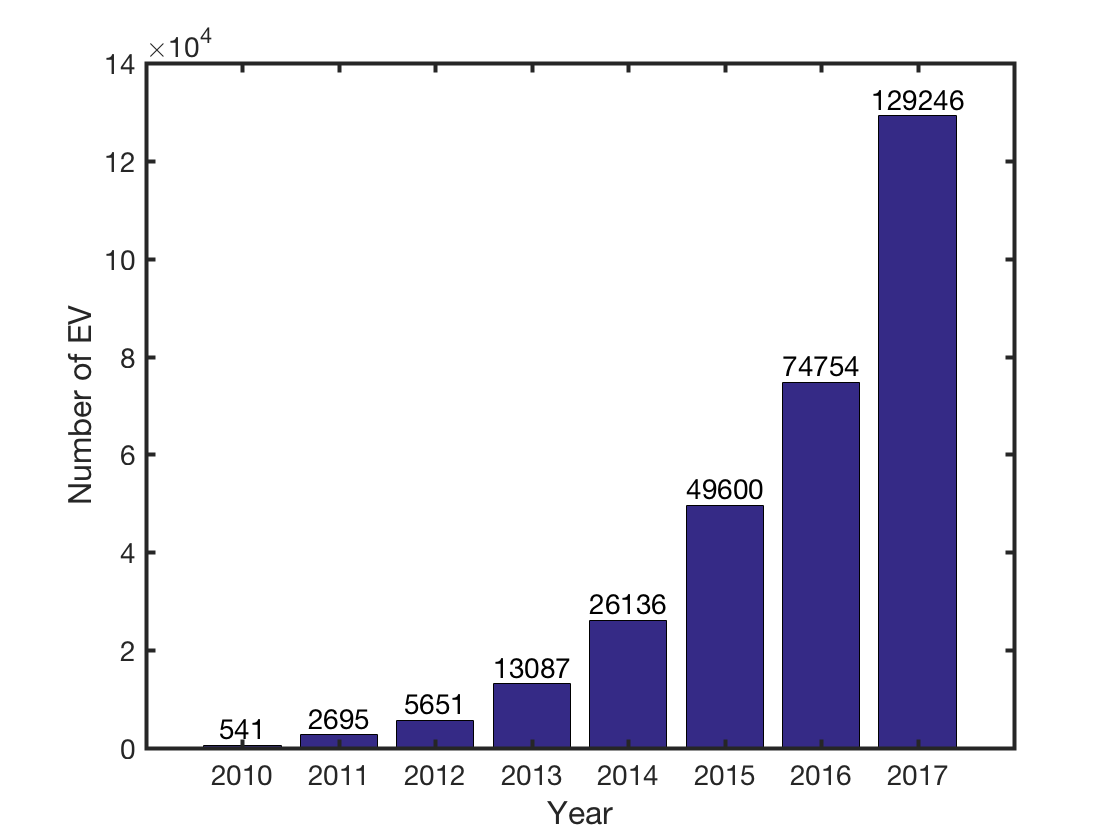
\includegraphics[width=0.95\linewidth]{Figures/Germany_EV_number}
	\caption{Cumulative registration of plug-in electric vehicles in Germany since 2010 \cite{KBA2017}}
	\label{fig:Germany_EV_number}
\end{figure}

By taking the EV number as \num{74754} in 2016 and \num{129246} in 2017, we performed the case studies and the results are shown by Figure \ref{fig:Germany_EV}. All the business cases reported profits, especially the cases where frequency control markets are coupled. However, it shall be noticed that our analysis has overlooked some factors which could make the business less profitable as they are shown here. One issue is that we use a determinate approach to simulate the EV driving behaviors which eliminated the risks of failing to deliver the frequency control services as planned. Alipour \textit{et. al.}\cite{Alipour2017} made a study on EV2G for frequency control services with a stochastic approach. It was found in a case where a profit of 7980 USD was expected, the conditional value-at-risk was 5720 USD, indicating the risking nature of such a business. In the outlook of this thesis, we proposed a stochastic method by using Markov chain to simulate the uncertain driving behavior of EVs and then the estimation of risk can be conducted. Nonetheless, while risk control against uncertainty is necessary for designing a specific project, it is beyond the focus for a study understanding the whole market value so is not included in our study.

Besides, it shall be noticed that implementing EV2G for frequency control is not a mature technology due to its complexity\cite{Peng2017}\cite{Shafie-Khah2015} \cite{Bessa2014}\cite{Bessa2013}, which implies a high research and development cost for the technology vendors. 

\begin{figure}[h!]
	\centering
	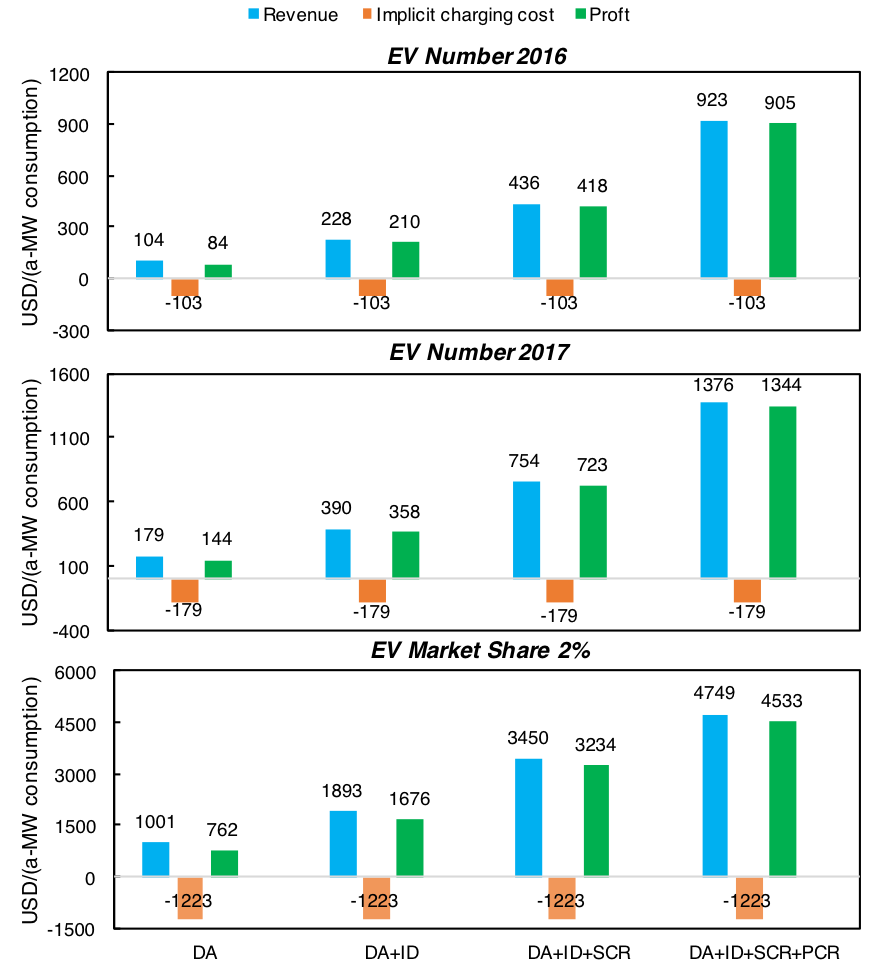
\includegraphics[width=0.95\linewidth]{Figures/Germany_EV_profit}
	\caption{Market Size and Profitability of EV2G in PJM Electricity Markets}
	\label{fig:Germany_EV}
\end{figure}


\subsubsection{Market Size and Profitability of EV2G  in PJM}
We performed the study in PJM power markets. Firstly it is found that which additional 300k EVs, it would gradually fall into supply shortage (Figure \ref{fig:EV_nan_percentageg-PJM}).

\begin{figure}[h!]
	\centering
	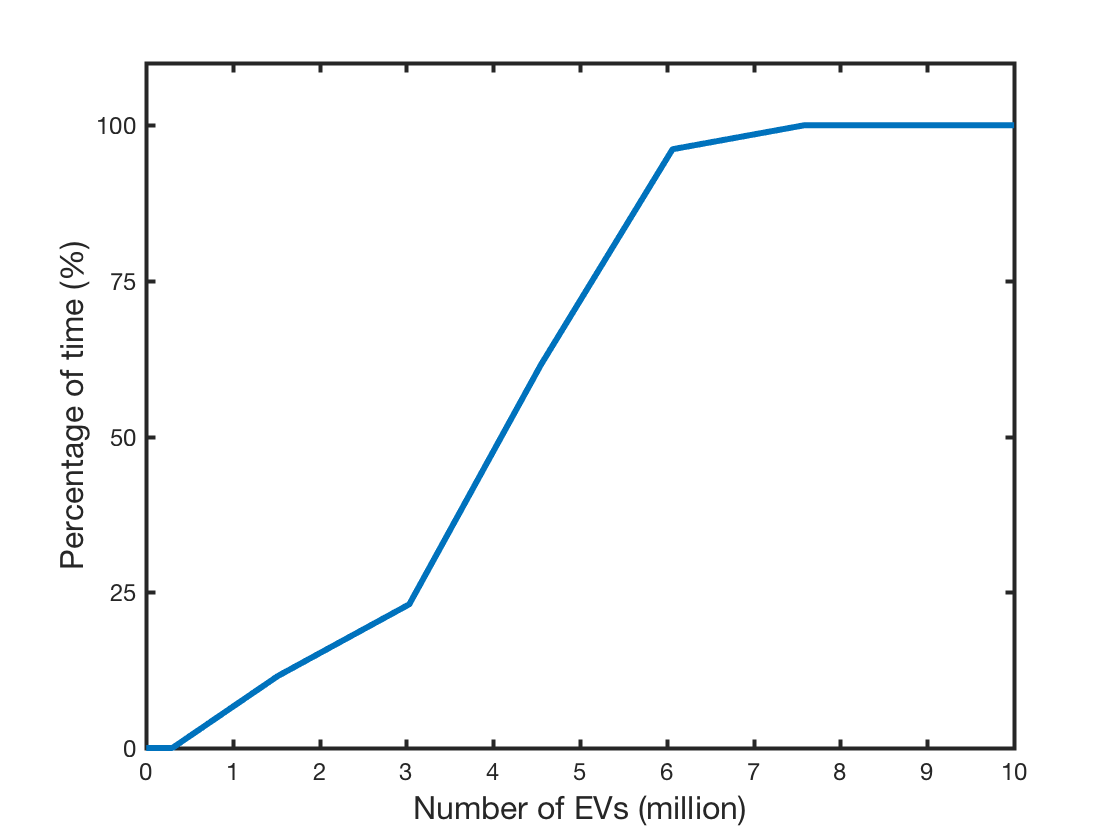
\includegraphics[width=0.95\linewidth]{Figures/EV_nan_percentage_PJM}
	\caption{Percentage of time when EV charging demand cannot be fulfilled in PJM}
	\label{fig:EV_nan_percentageg-PJM}
\end{figure}

Since the geographic coverage of PJM is not strictly corresponding to the administrative divisions, it is a complex task to get the official number of EVs in PJM with the public data. Therefore, we projected the number in Germany to PJM by their ratio of household number. That means, in the corresponding scenarios, the EV ownership per household is identical in Germany and PJM. We took this approach to make an indication of the market value, which however shall be viewed with caution that it may deviate from real conditions.

\begin{figure}[h!]
	\centering
	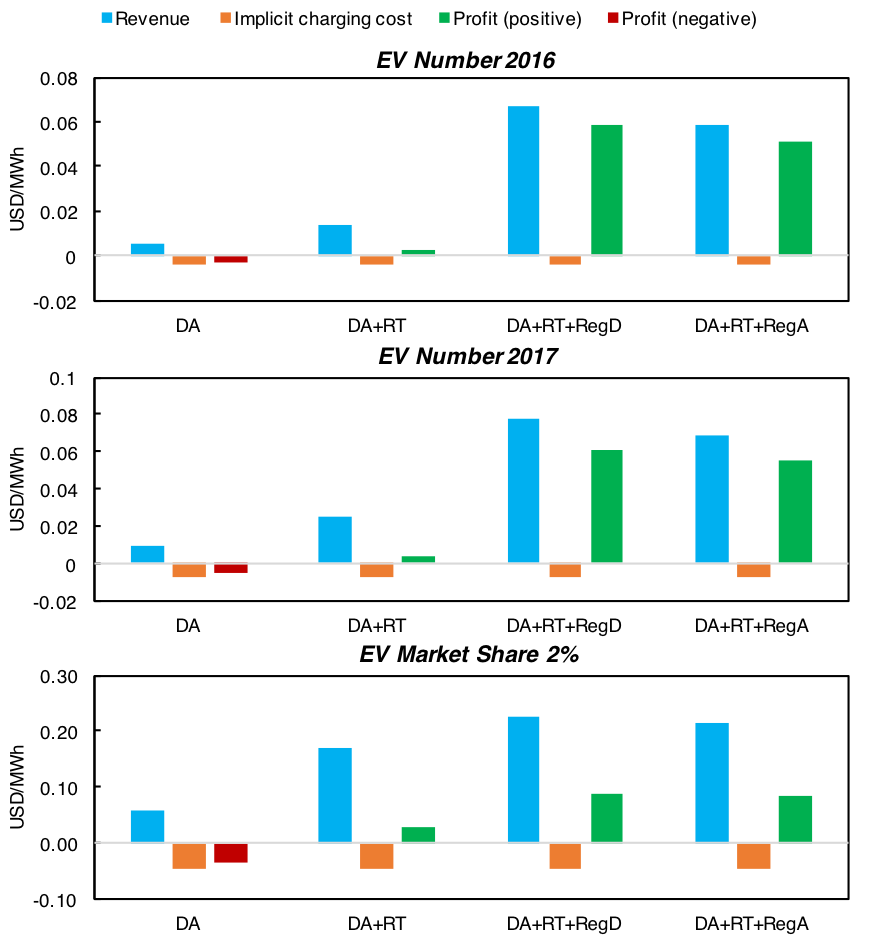
\includegraphics[width=0.95\linewidth]{Figures/PJM_EV_profit}
	\caption{Market Size and Profitability of EV2G in PJM Electricity Markets}
	\label{fig:PJM_EV}
\end{figure}

Figure \ref{fig:PJM_EV} summarizes the results of cases in PJM. Compared the results in Germany markets, it can be found that while profits in energy-only cases are closed, the profits with frequency regulation are much higher in PJM than the Germany, which again reveals the adversity against flexibility resources in Germany frequency control markets.

 
\subsubsection{Market Size and Profitability of EV2G  in NSW}

\textit{(An issue was found related to this case while analyzing the data, so the results will be ready later.)}



\subsection{Impact analysis of changing market conditions}
\label{sec:impact-market-condition}

\subsubsection{Model validation}
As is introduced in Section \ref{sec:market-simulation}, the market simulation module was designed to generate price scenarios with changed market conditions so that we can analyze the future trend of market value, or at least the potential impacts of certain key factors. 

The module is developed using the methodology in Section \ref{sec:market-simulation}. It is trained and validated by day-ahead price and generation data in Germany in 2016. 

In order to get the parameters of the model we first collect the Germany day-ahead market in 2016, shown as Figure \ref{fig:merit-orignal}.

\begin{figure}[h!]
	\centering
	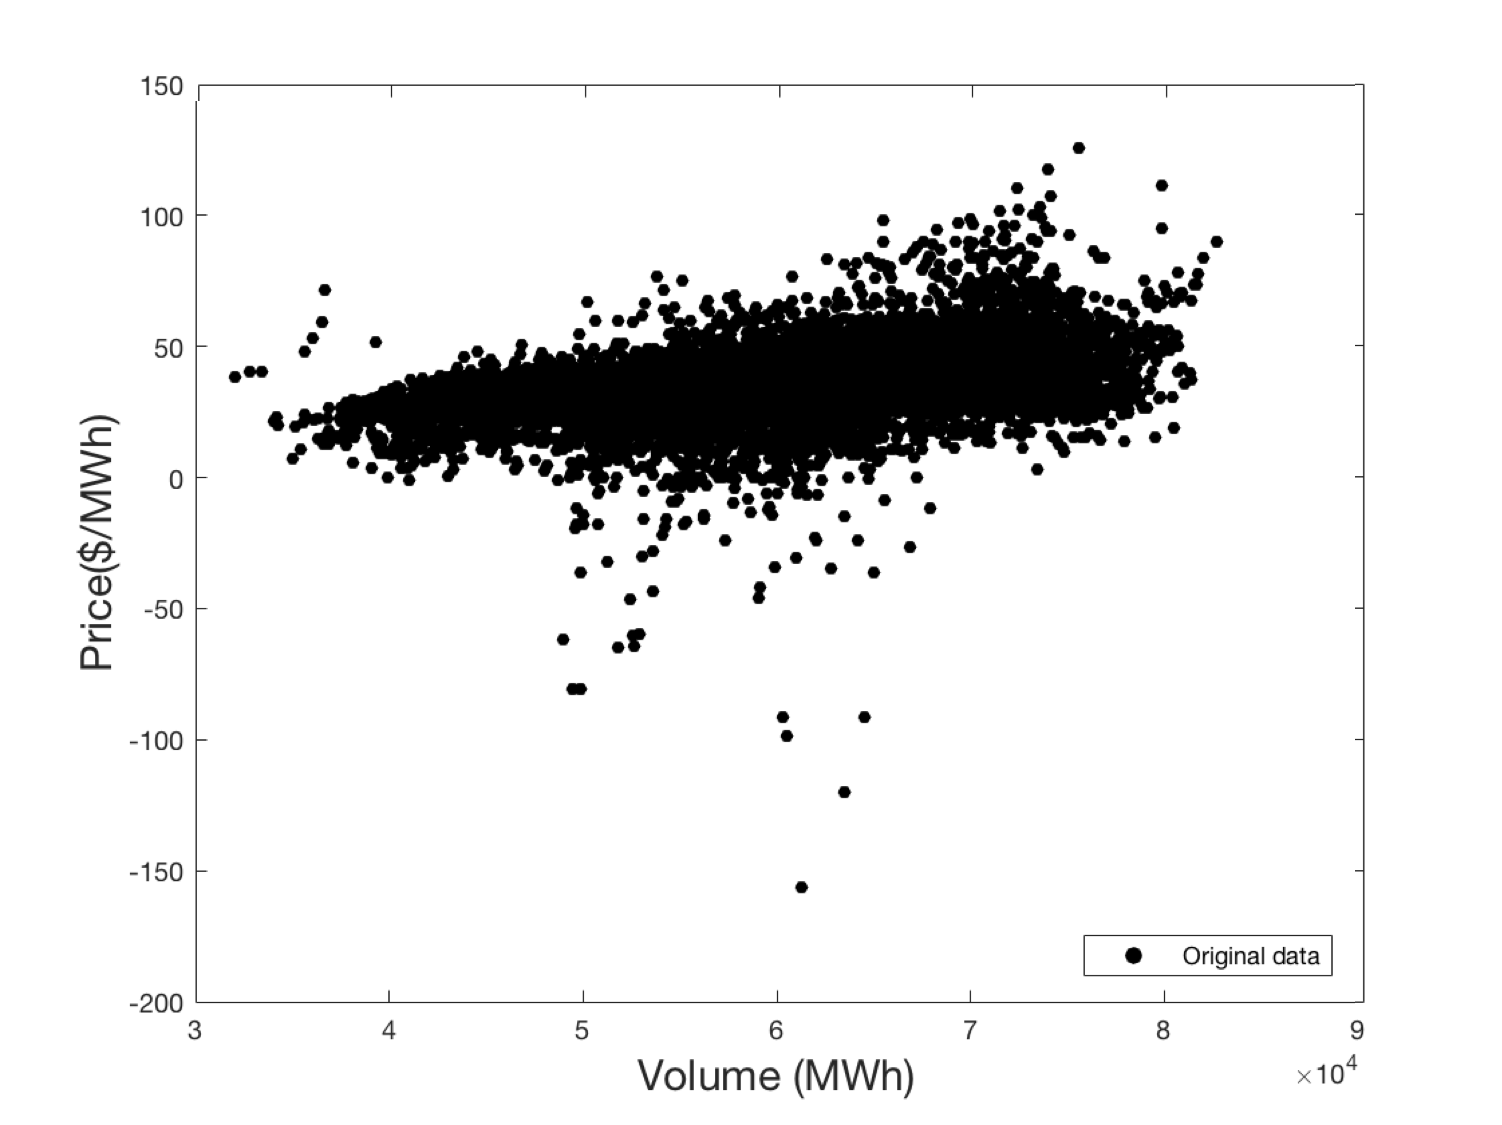
\includegraphics[width=0.95\linewidth]{Figures/Merit-order-original}
	\caption{Germany day-ahead price-volume data in 2016}
	\label{fig:merit-orignal}
\end{figure}

It clearly shows that the pattern of merit-order effect is not recognizable from the original data mainly due to the disturbs of variable renewable generation which has raised significantly in past years. This prevents us from directly applying the merit-order models developed by previous studies\cite{He2013}\cite{Grunewald2012a}. Therefore, we applied the algorithm described in Section \ref{sec:market-simulation} which take into account the renewable generation and bounded flexibility of conventional generations. Figure \ref{fig:merit-transformed} shows the transformed pattern of data where a clearer merit-effect is identifiable. Figure \ref{fig:merit-classified} projects the classification to the original data distribution and it can be seen that the algorithm has successfully separated the data points where the price was driven to be higher or lower than average level due to the uplift effects introduced in \ref{sec:market-simulation}. 

\begin{figure}[h!]
	\centering
	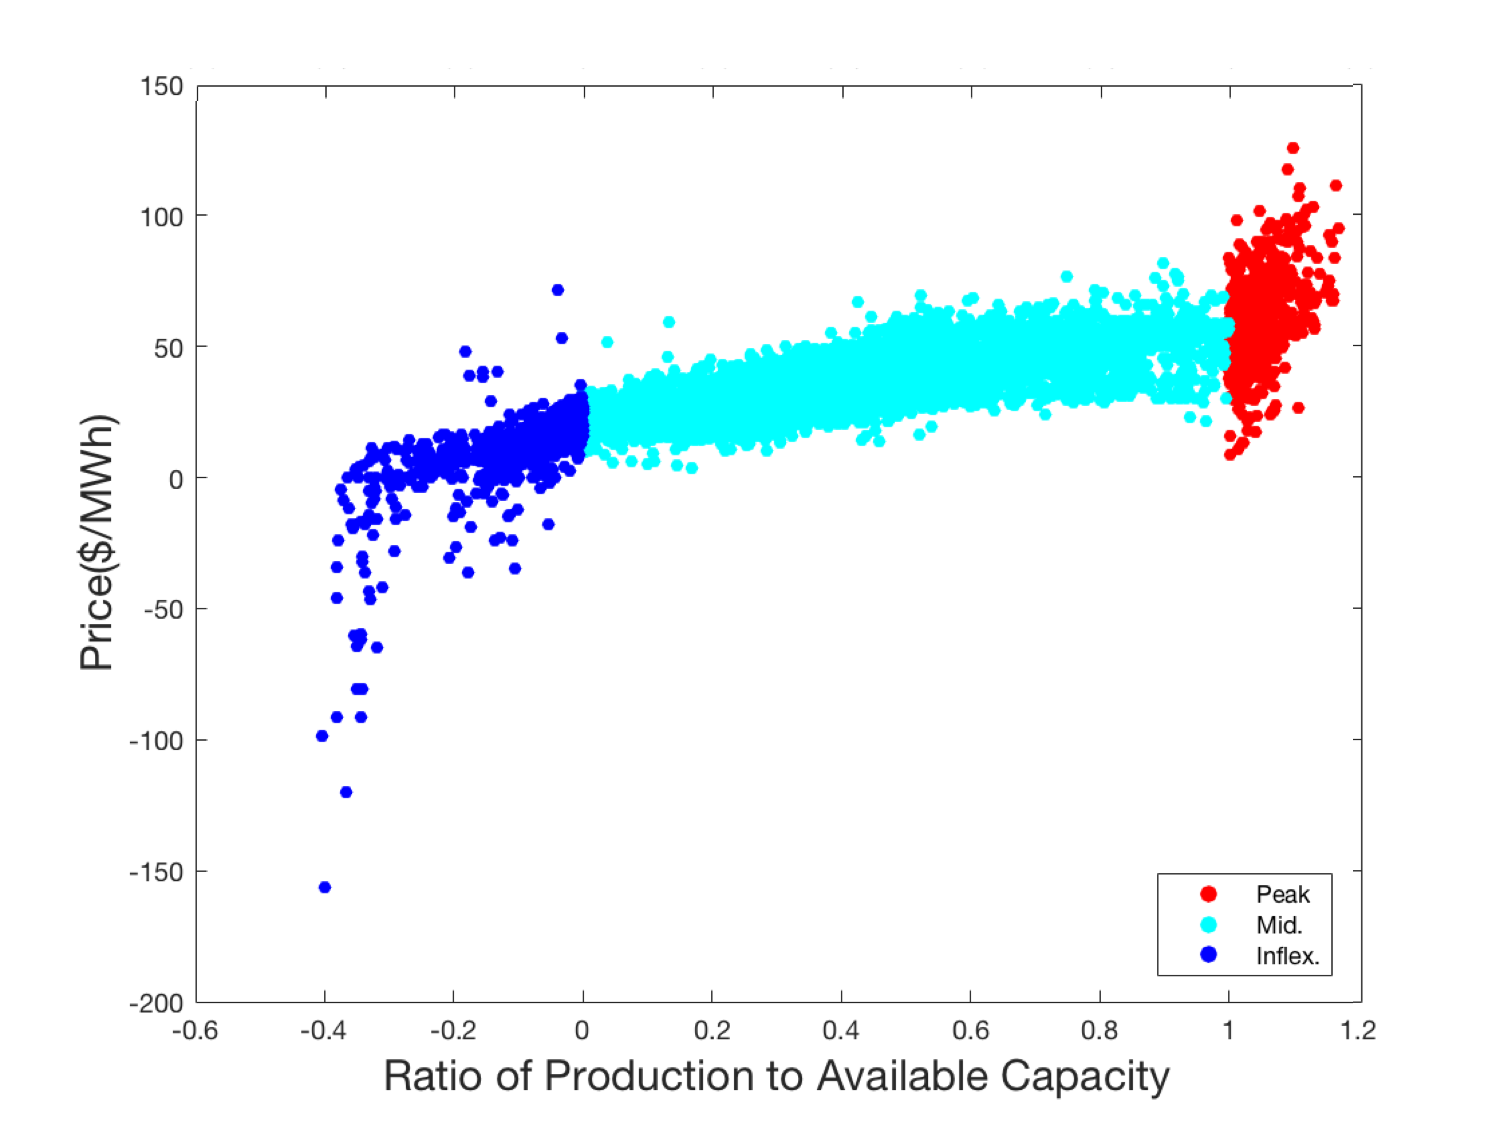
\includegraphics[width=0.95\linewidth]{Figures/Merit-order-transformed}
	\caption{Transformed pattern of Germany day-ahead price-volume data in 2016}
	\label{fig:merit-transformed}
\end{figure}
\begin{figure}[h!]
	\centering
	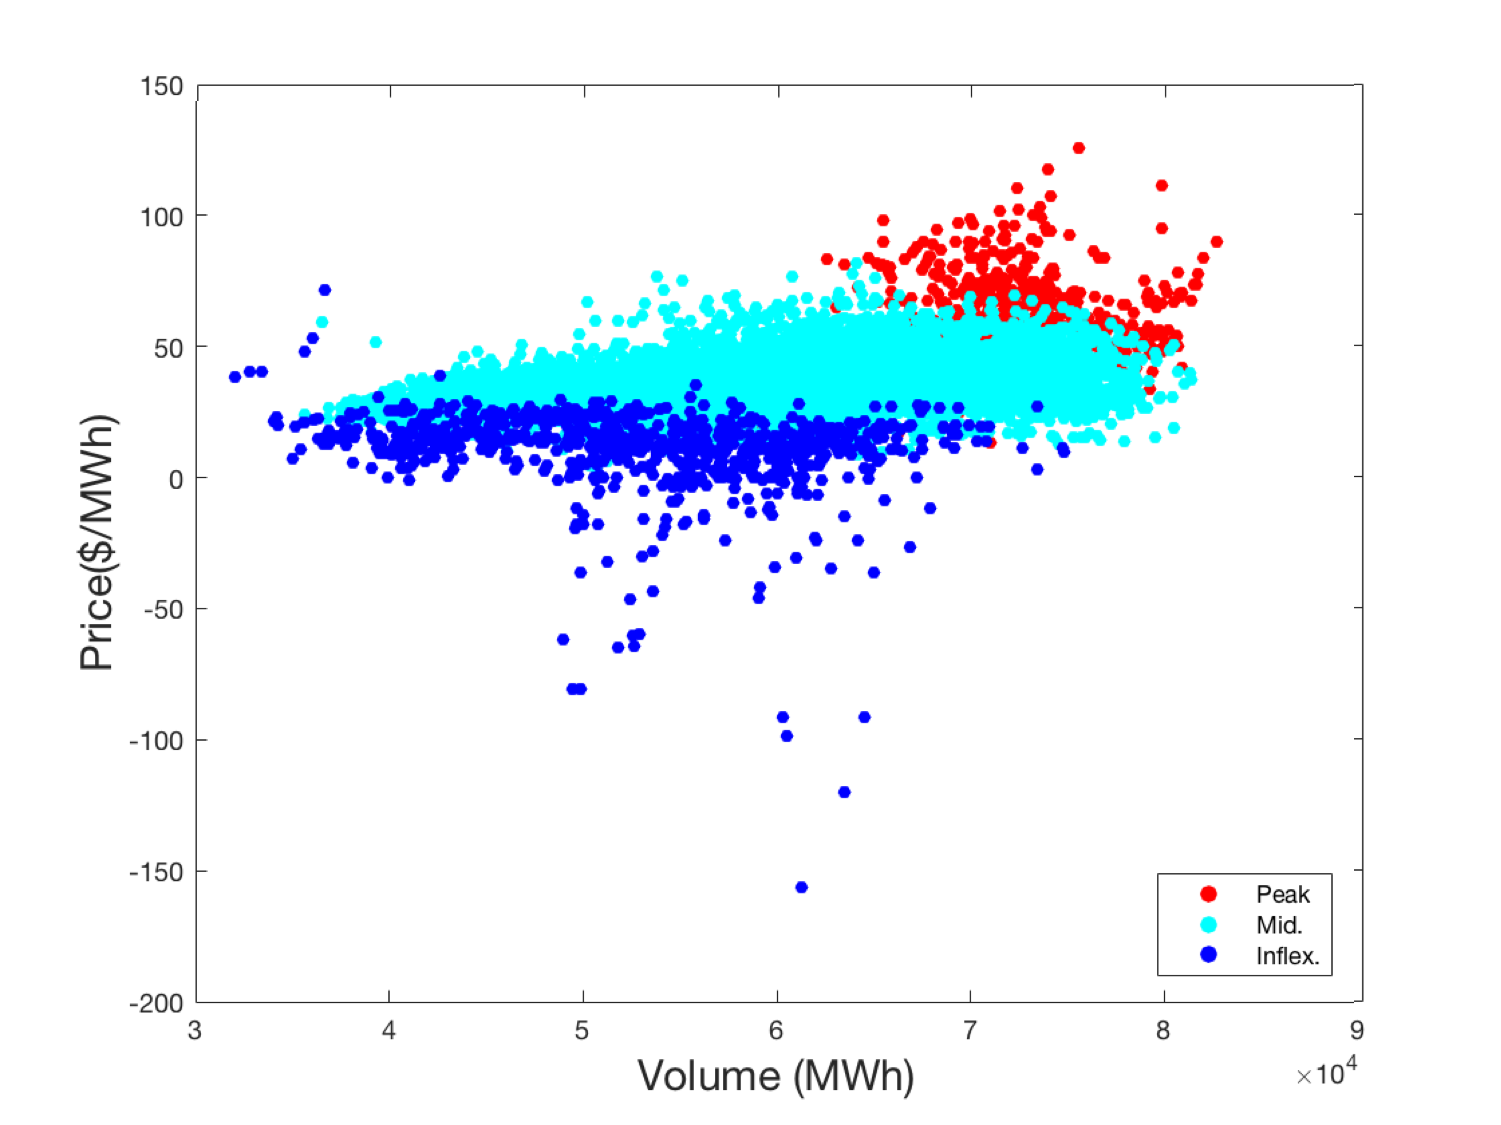
\includegraphics[width=0.95\linewidth]{Figures/Merit-order-classified}
	\caption{Classification of Germany day-ahead price-volume data in 2016}
	\label{fig:merit-classified}
\end{figure}

Thereafter, we fitted the transformed data pattern with piece-wise function, as is shown by Figure \ref{fig:merit-fitted}. The distribution of error between the fitted price and actual price is illustrated by Figure \ref{fig:merit-error}.

\begin{figure}[h!]
	\centering
	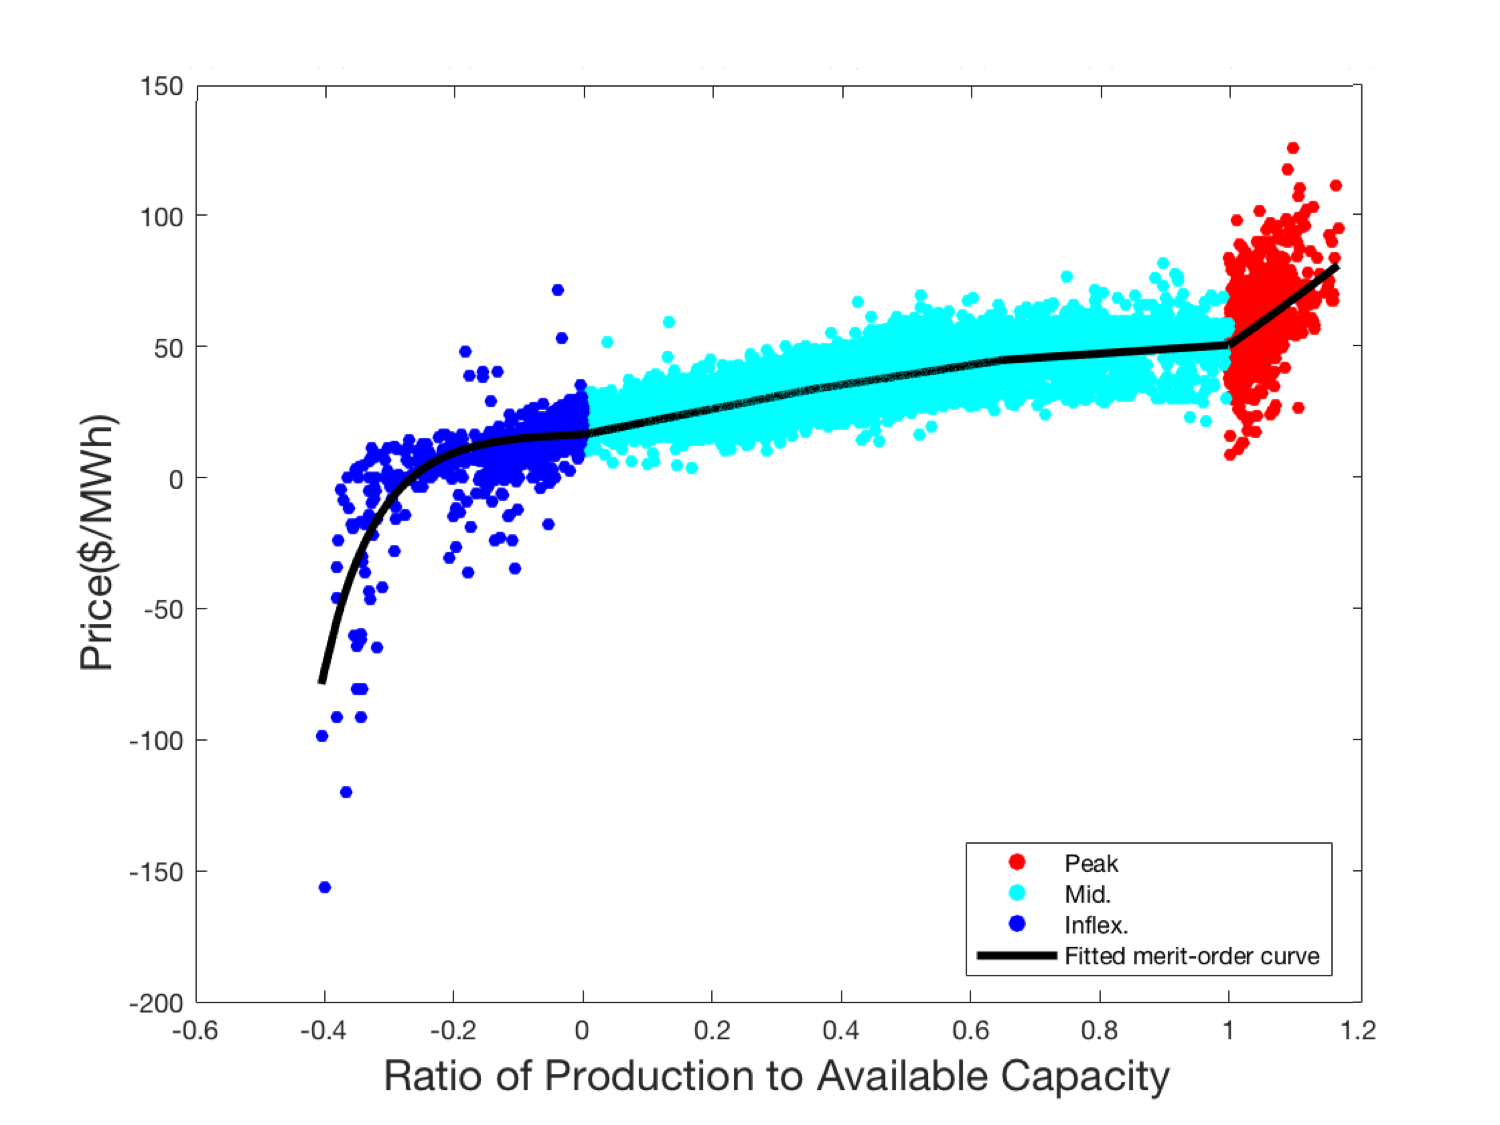
\includegraphics[width=0.95\linewidth]{Figures/Merit-order-fitted}
	\caption{Fitted merit-order curve with Germany day-ahead price-volume data in 2016}
	\label{fig:merit-fitted}
\end{figure}

\begin{figure}[h!]
	\centering
	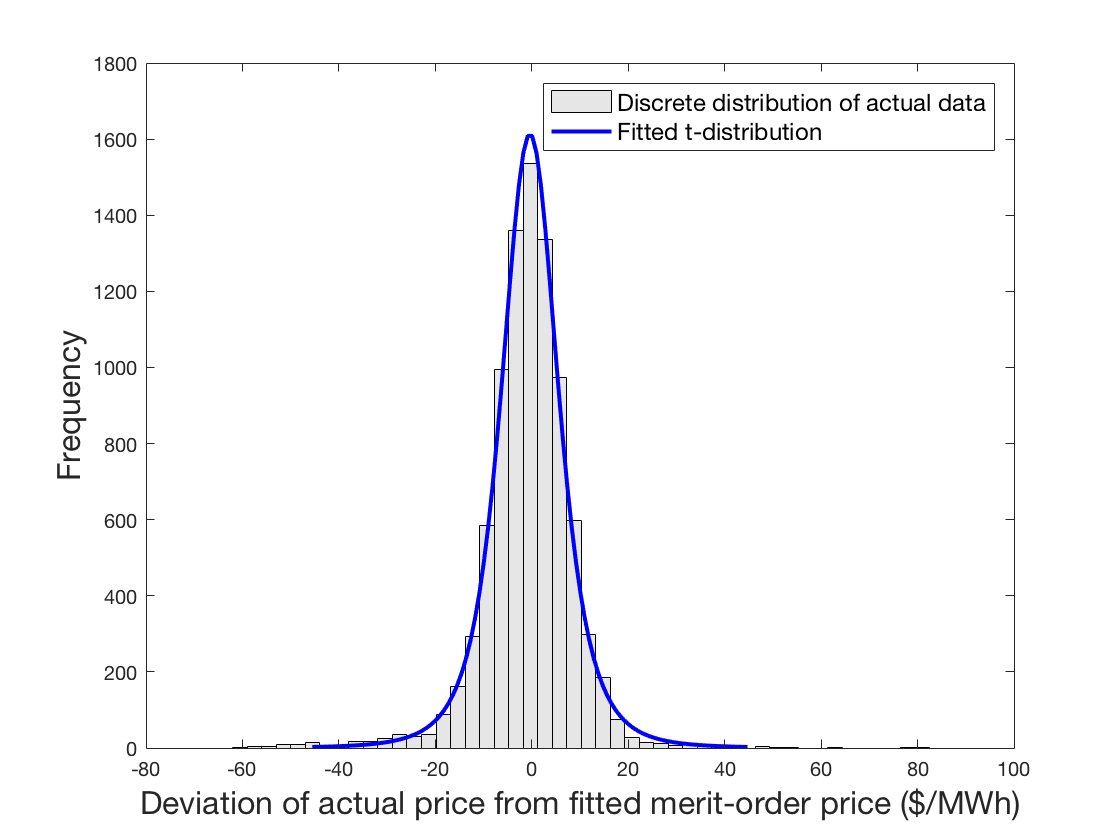
\includegraphics[width=0.95\linewidth]{Figures/4_Error-distribution}
	\caption{Distribution of errors between fitted merit-order price and actual price}
	\label{fig:merit-error}
\end{figure}

As we can see from Figure \ref{fig:merit-fitted}-\ref{fig:merit-error}, the fitted merit-order price eliminated the stochastic movement of the price. If we simulated the price movement merely with the merit-order model, it will show a smoothed curve where the drastic jumps of price cannot be captured, which can be demonstrated by Figure \ref{fig:price-example}.

\begin{figure}[h!]
	\centering
	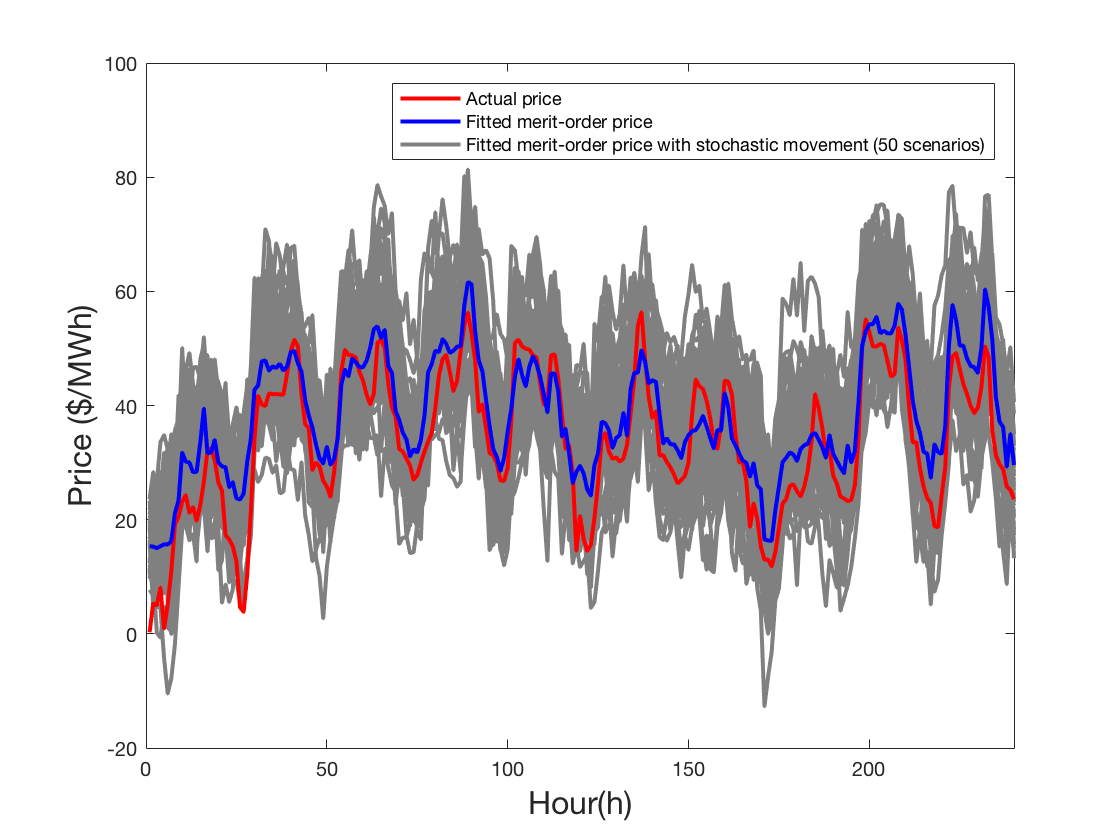
\includegraphics[width=0.95\linewidth]{Figures/5_Example-simulated_price}
	\caption{Generated price scenarios}
	\label{fig:price-example}
\end{figure}

Although it might suffice the needs of valuing a conventional generation resources, the elimination of stochastic price movement would reduce the value of arbitrage greatly as is shown by Figure \ref{fig:model-validation}.

\begin{figure}[h!]
	\centering
	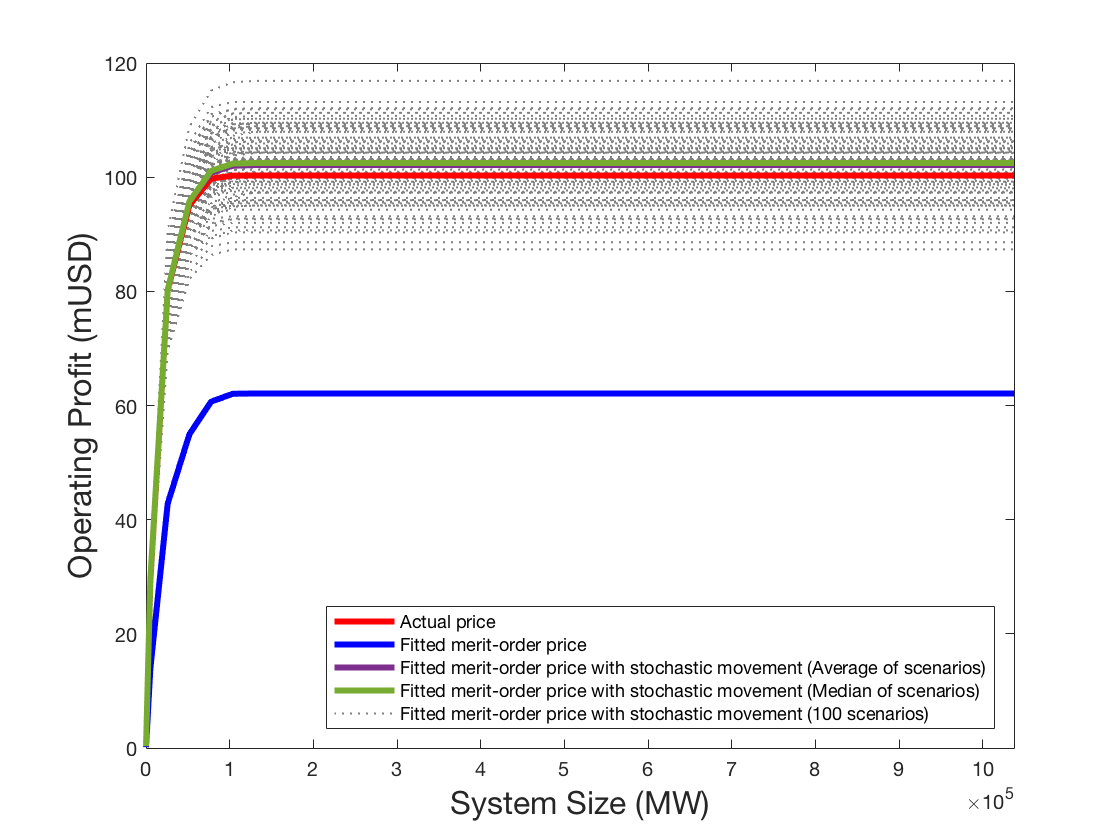
\includegraphics[width=0.95\linewidth]{Figures/6_Model_Validation}
	\caption{The revenue with different price scenarios}
	\label{fig:model-validation}
\end{figure}

Therefore, we applied the seasonal auto-regressed moving-average (SARMA) model as is described in \ref{sec:market-simulation} to simulate the stochastic components of the price. The estimated parameters of the SARMA model is listed in Table \ref{tab:SARMA}. Thereafter, we conducted Monte-Carlo simulations to generate a number of scenarios of the stochastic parts of price, which are then added to the determinate trends calculated by the merit-order model. The final simulated price scenarios are illustrated by the grey lines in Figure \ref{fig:price-example}. Using these generated price profiles, we calculated the revenue for 10 scenarios and compare the average value to the value obtained with actual price signal, which shew a perfect fitness in Figure \ref{fig:model-validation}. 

\begin{table}
	\label{tab:SARMA}
	\centering
	\begin{tabular}{|c c|}
		\hline
		\multicolumn{2}{|c|}{SARMA parameters}\\
		\hline
		\hline
		$\phi_1 = 1.811$ & $\theta_1 = -1.063$ \\
		$\phi_2 = -0.813$ & $\theta_{24} =0.692$ \\
		$\phi_{24} = 0.090$ & $\theta_{168} = -0.600$ \\
		$\phi_{168} = 0.692$ & \\
		\hline
	\end{tabular}
\caption{Parameters of the stochastic price movement of SARMA models}
\end{table}

\newpage
\subsubsection{Impact of renewable penetration}

\subsubsection{Impact of increasing flexibility on generation side}

\subsection{Impact of increasing flexibility on demand side}

\subsection{Sensitivity analysis}
\subsubsection{Limited predictibility}

\subsubsection{Responsive price}

\subsubsection{Database}

\subsubsection{Locational price}

\subsubsection{Sensitivity analysis of other parameters}





